\subsection{ESG Considerations in Investment Analysis}

\begin{definition} Types of Ownership:
\begin{enumerate}[label=\roman*.]
\setlength{\itemsep}{0pt}
\item \hlt{Dispersed Ownership}: numerous shareholders, none have ability to individually exercise controls
\item \hlt{Concentrated Ownership}: an individual or group with ability to exercise control
\end{enumerate}
\end{definition}

\begin{remark} Degree of Control:\\
Degree of share ownership is not reliable indicator of concentration of control.
\begin{enumerate}[label=\roman*.]
\setlength{\itemsep}{0pt}
\item \hlt{Horizontal Ownership}: companies with mutual business interests (i.e., key customers or suppliers) have cross-holding share agreements with each other. Facilitate strategic alliances and long-term relationship.
\item \hlt{Vertical Ownership}: company or group that has control in two or more holding companies, which in turn have controlling interests in various operating companies.
\end{enumerate}
Dual-class shares may give one class of shareholder superior voting rights, another class with fewer voting rights.
\end{remark}

\begin{remark} \hlt{Conflicts with Different Ownership Structures}
\begin{enumerate}[label=\roman*.]
\setlength{\itemsep}{0pt}
\item Dispersed ownership, dispersed voting power: weak shareholders, strong managers. Principal-agent conflict likely; shareholders want value maximised, managers use firms resources to own advantage. Mitigated with presence of controlling shareholders.
\item Concentrated ownership, concentrated voting power: strong shareholders, weak managers. Control of board of directors, effectively control and monitor management. Principal-principal conflict; controlling owners take advantage of firm resources to detriment of minority owners.
\item Dispersed ownership, concentrated voting power: controlling shareholders gain control over minority shareholders with pyramid structures or dual-class shares. Controlling shareholders monitor management.
\item Concentrated ownership and dispersed voting power: presence of voting caps, where voting rights of large share positions are restricted. Sovereign countries may enact this to discourage foreign investors from taking controlling position in a company belonging to an industry considered important.
\end{enumerate}
\end{remark}

\begin{remark} \hlt{Types of Influential Shareholders}
\begin{enumerate}[label=\roman*.]
\setlength{\itemsep}{0pt}
\item Banks: if bank is both lender and shareholder to a firm, may use influence to encourage firm to take out expensive loans from the bank. Corporate governance controls to ensure bak does not take advantage of its role as lender at expense of other shareholders.
\item Families: one family controlling multiple companies through interlocking directorates (individual to sit on boards of numerous companies). Principal-agent issues reduced, but difficult to recruit quality outsiders for management. Lack of concern for minority shareholders, minimal transparency and low accountability.
\item State-Owned Enterprises (SOE): partly owned by government and trades on exchange. Seek to provide social benefits to public rather than focusing only on shareholder value maximisation.
\item Institutional Investors: can represent large portion of equity ownership, wield shareholder rights with expertise because of their experience and resources. Typically pressure firm's management and board to act in the interest of shareholders.
\item Group Companies: achieve outsized amount of control through cross-holding of shares via vertical and horizontal ownership. Difficult for outsiders to acquire shares, increases potential for firms to participate in related-party transactions that do not advantage minority shareholders.
\item Private-Equity Firms: may bring beneficial changes to portfolio firm's corporate governance, i.e., performance-based compensation for managers, addition of corporate codes.
\item Foreign Investors: demand greater accountability and transparency, especially in emerging markets. Minority shareholders benefit when company decides to cross-list its shares in a country that has greater protection for investors and higher levels of transparency.
\item Mangers and Board Directors: interests more aligned with those of other shareholders, more likely to use firm's resources to boost profitability over long term. Potential for insiders to use their ownership to protect own interests instead of other shareholders.
\end{enumerate}
\end{remark}

\begin{remark} \hlt{Effect of Ownership Structure on Corporate Governance}
\begin{enumerate}[label=\roman*.]
\setlength{\itemsep}{0pt}
\item Director Independence: directors wth no material ownership with the company with regard to employment, ownership, or renumeration. Important in countries with dispersed ownership, where principal-agent problem is greater, hence board monitoring of managers is key. Portion of independent directors on boards has increased in aftermath of corporate scandals.
\item Board Structures: either one-tier board (internal and external directors), or two-tier board (management board overseen by supervisory board). Supervisory board determine management compensation, supervising external auditors, reviewing financial records. Stakeholder representatives may sit on board.
\item Special Voting Arrangement: advantage for minority shareholders to act on board nomination and election
\item Corporate Governance Codes, Laws, Listing Requirements: some countries have national corporate governance codes, or use company law or regulation, stock exchange listing requirements to require firms to adopt best practices or explain why they have not
\item Stewardship Codes: voluntary codes that encourage investors to exercise legal rights and increase their level of engagement in corporate governance. In UK, the code includes a duty for institutional investors to monitor their invested companies.
\end{enumerate}
\end{remark}

\begin{remark} \hlt{Effectiveness of Board Policies and Practices}
\begin{enumerate}[label=\roman*.]
\setlength{\itemsep}{0pt}
\item Structure of Board of Directors: Analyse on whether the board is appropriate in light of its accountability to shareholders, and its oversight and representation. CEO duality occurs when the chairperson of the board is also CEO; raises concerns that chairperson's oversight and monitoring may not be effective.
\item Board Independence: majority of board members should be independent; this prevent management from self-serving behaviour, and lowers investor perceptions of risk.
\item Board Committee: to consider if key committees reporting to financial reporting, management selection, and compensation are sufficiently independent.
\item Skills and Experience of Board: board members to have industry-specific experience and skills, and have board expertise needed to function efficiently in board member role. Board members also to have some previous exposure to concerns on ESG risks. Long-tenured board member will have strong knowledge of operations of the firm's management and business operations, but may be resistant to beneficial change.
\item Composition of Board: small, diverse board is more effective. Diversity refers to characteristics such as age, gender, length of tenure, education, culture, and place of birth.
\item Other Board Evaluation Considerations: boar structure and committees, culture of the board, interaction with management, its effectiveness, and its leadership. 
\end{enumerate}
\end{remark}

\begin{remark} \hlt{Executive Compensation}\\
To have executive compensation tied to KPIs. 
\begin{enumerate}[label=\roman*.]
\setlength{\itemsep}{0pt}
\item Clawback Policies allow firm to reclaim past compensation if inappropriate conduct comes to light later.
\item Say-on-pay rules gives stakeholders the opportunity to vote on executive compensation.
\end{enumerate}
\end{remark}

\begin{remark} \hlt{ESG-Related Risks and Opportunities} 
\begin{enumerate}[label=\roman*.]
\setlength{\itemsep}{0pt}
\item Materiality and Investment Horizon: to evaluate the materiality (impact on company operations, financial performance, valuation of securities) of underlying data. Also to consider the investment horizon and holding period when deciding ESG factors to consider in the analysis.
\item Relevant ESG-Related Factors: to determine which ESG specific factors are most relevant to the particular industry and firm. Approaches to identify company ESG factors include:
\begin{enumerate}[label=\arabic*.]
\setlength{\itemsep}{0pt}
\item ESG Data Providers: provides information in form of rankings, scores, and quantitative analysis.
\item Industry Organisations: not-for-profit groups providing information on ESG factors, which includes IIRC, SASB. These organisations work to promote standardised corporate disclosures of ESG issues.
\item Proprietary Methods: own judgment and tools used to research ESG data from published reports, government organisations, and other sources. Company-specific ESG data gathered from annual reports, corporate citizenship or sustainability reports, proxy reports, regulatory filings.
\end{enumerate}
\end{enumerate}
\end{remark}

\begin{remark} \hlt{ESG Security Analysis}
\begin{enumerate}[label=\roman*.]
\setlength{\itemsep}{0pt}
\item Fixed Income Analysis: focus on ESG factor downside risk ad on stranded assets. Effect of lawsuit on credit ratios, cash flow, liquidity are considered.
\item Equity Analysis: both upside and downside impact are factored. Involves forecasting financial metrics and ratios, adjusting valuation model variables, using sensitivity and/or scenario analysis.
\item Green Bond: fixed income, used to fund projects related to environment. Same recourse, credit ratings as issuer's other bonds, with intended use of proceeds. Valuation similar to conventional bond, except with a price premium. Concern of greenwashing.
\end{enumerate}
\end{remark}

\begin{figure}[H]
\centering
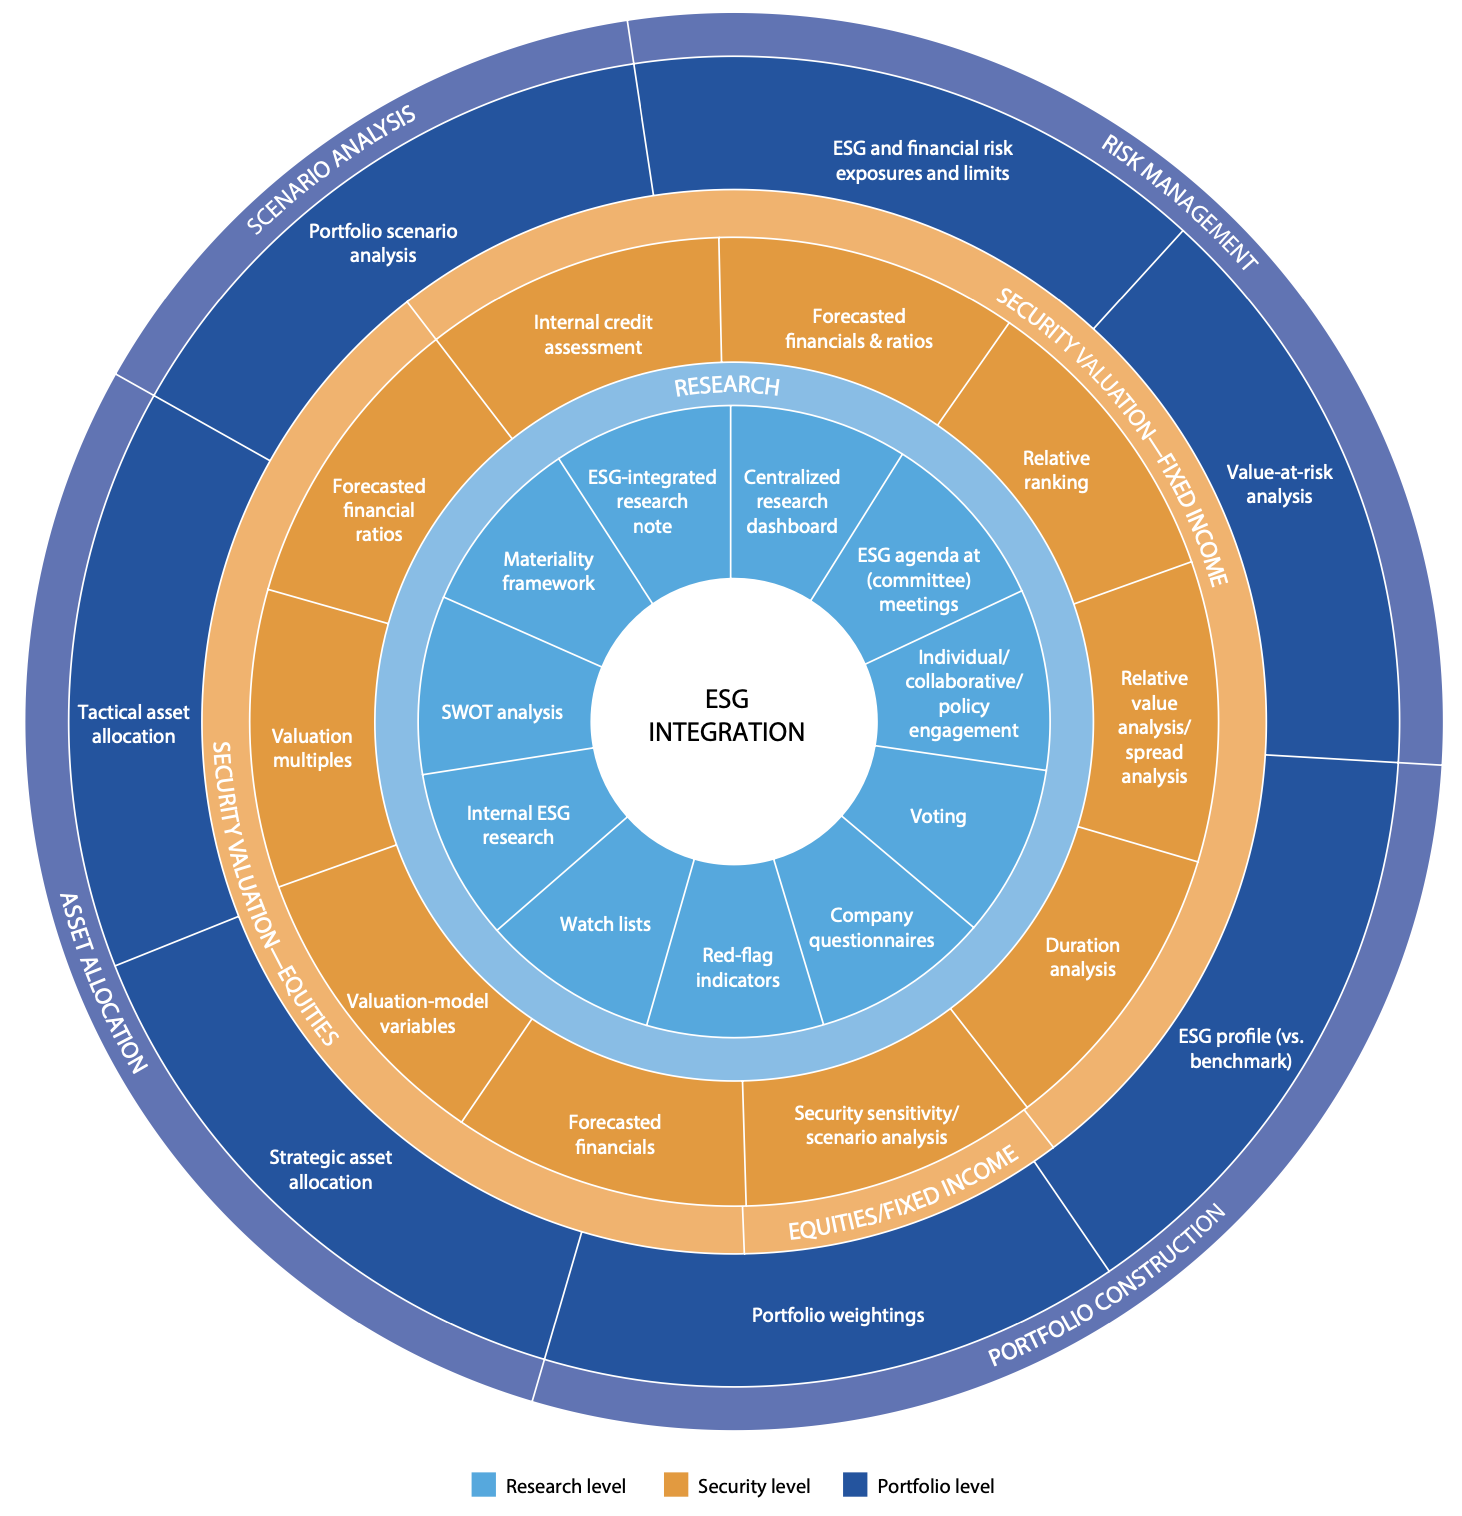
\includegraphics[scale=0.6]{/corpissuer/esgint}
\caption{ESG Integration Framework}
\end{figure}
